\section{Results and Interpretation}


\subsection{Performance}

We searched in the source code of Android framework since version 4.0 for string ``\verb|/dev/random|'' and found no reference to it. We also captured all read operation on \verb|/dev/random| in a daily use of a Nexus 7 tablet since boot, and found only once, process \verb|wpa_supplicant| read from it. It was a WPA authenticator and it used \verb|/dev/random| to initialize its own PRNG.

All Android applications who want high quality random number are recommended to use a Java class named SecureRandom, which on initialization read from \verb|/dev/urandom| to seed its generator.

These results indicate that the performance issue cannot be attributed to blocking read of \verb|/dev/random| since there are nearly none.

There may be some links between the entropy collecting routine and the poor performance. We noticed that since Linux kernel 3.7, the input event entropy source handler in random.c source code has been restructured \cite{commit43} to improve the performance on multitouch devices by batching the input events. Some developers commenting on Issue 42265 also suggested that the performance issue is due to suboptimal order of event process and entropy accumulation. We cannot tell if there would be any improvement since we did not successfully install a kernel later than 3.7 on our devices, but we do suggest users keep their software up-to-date since the changes are quite reasonable and promising.

\subsection{Security}

\subsubsection{Entropy Sources}
\begin{figure*}[t]
\begin{center}
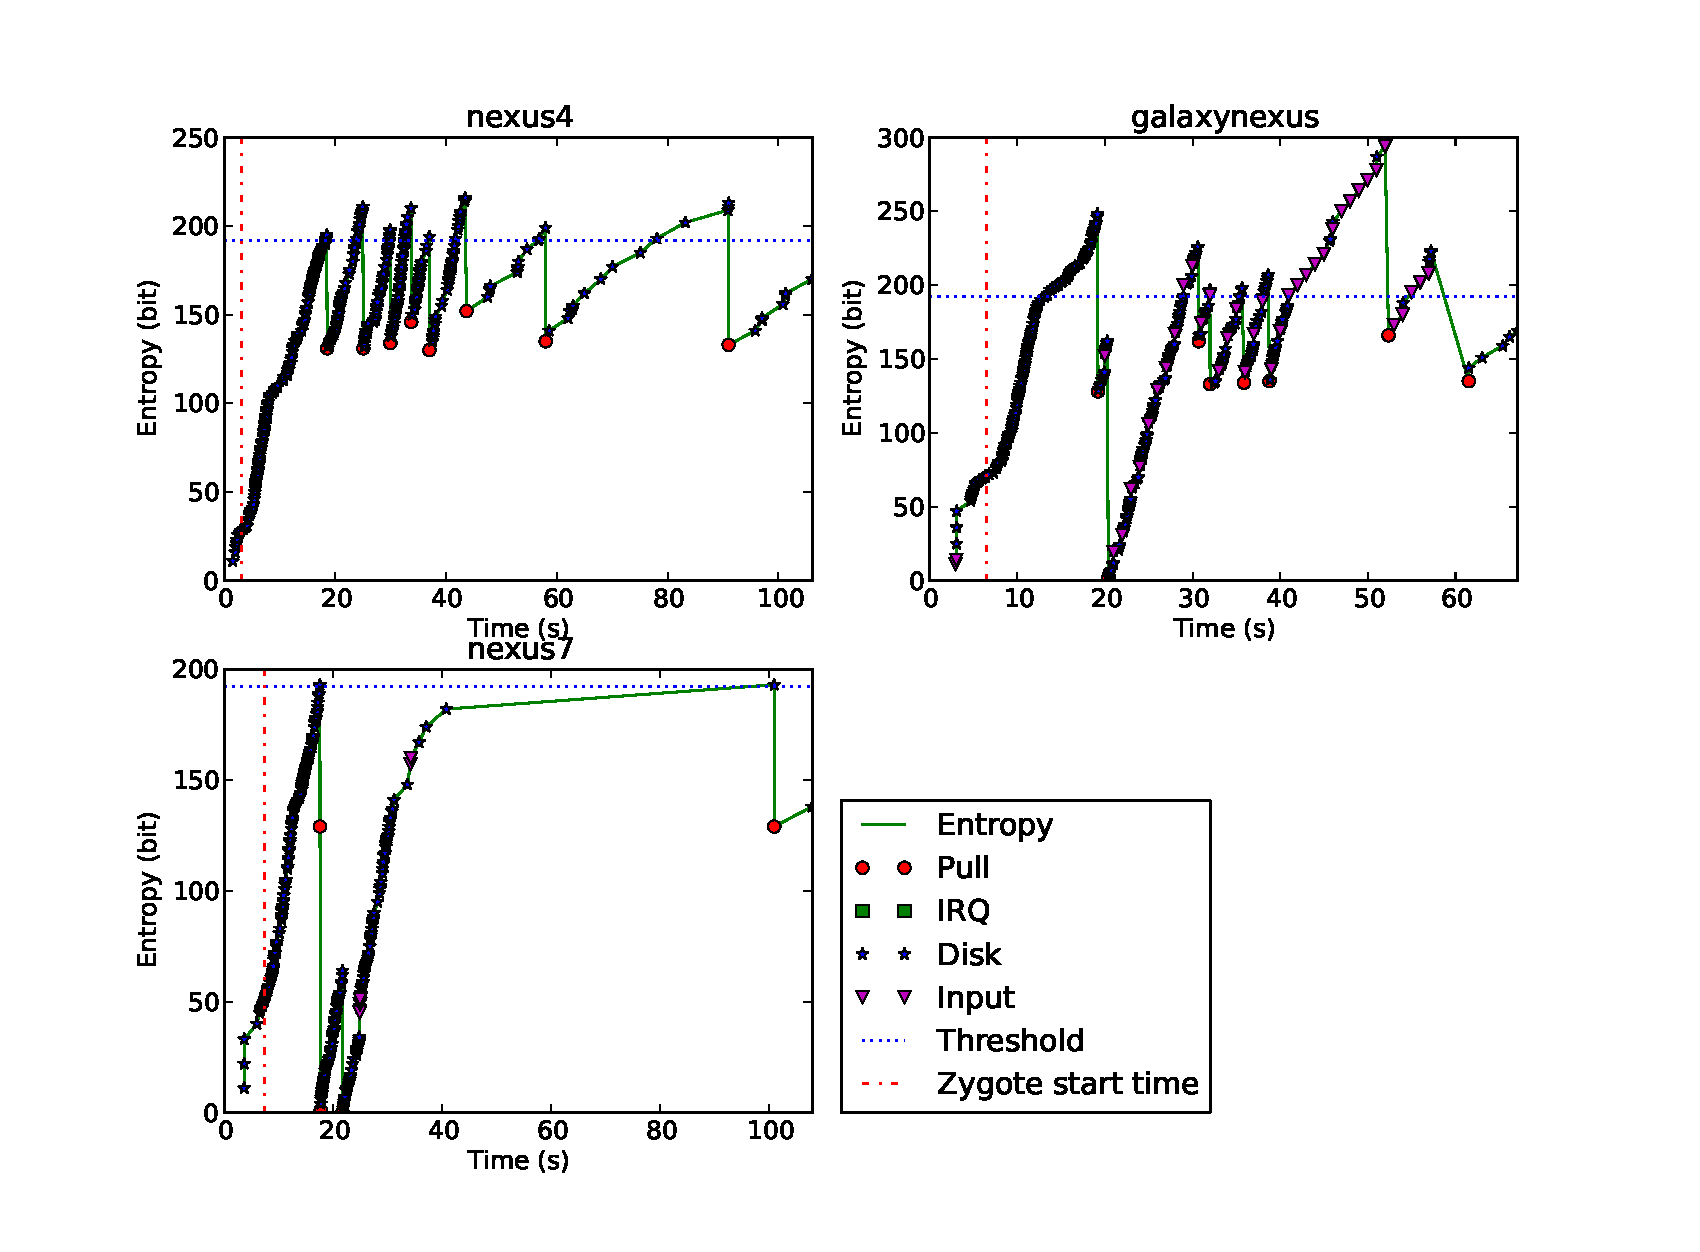
\includegraphics[scale=0.6]{entropy.eps}
\end{center}
\caption{{\bf Amount of Entropy Over Time:} The three devices shows different profiles on entropy accumulation, but their entropy crosses the 192 threshold quickly enough before the user interface is load up. Also note that when Zygote starts the entropy does not cross 192, thus no entropy is mixed into \texttt{/dev/urandom|}   }
\label{figentropy}
\end{figure*}

\begin{table}
\begin{center}
\begin{tabular}{|l|c|}
\hline
\bf Device & \bf Full Boot Time (s) \\
\hline
Nexus 4 & ?? \\
\hline
Nexus 7 & 24.8 \\
\hline
Galaxy Nexus & ??\\
\hline

\end{tabular}
\end{center}
\caption{{\bf Full Boot Time:} The time it takes from the kernel is loaded to the Android desktop launcher is brought up.}
\label{tblboottime}
\end{table}

Figure \ref{figentropy} suggests that the Android devices have sufficient source of entropy. The entropy contributed merely by disk events is enough to have \verb|/dev/urandom| properly seeded before any user applications can run.


\subsubsection{User Applications}

Figure \ref{figentropy} and \ref{tblboottime} show that the time when the user could start the first application is after the time when the amount of entropy first crossed the 192 threshold, which means the first read from \verb|/dev/urandom| will cause the non-blocking pool extract at least 10 bytes (\verb|EXTRACT_SIZE| defined in random.c). The 80 bits entropy is enough to prevent any attacker trying to predict the random number. There will be more entropy mixed in when user touches or slides on the screen as shown in table 3. If it is the first boot, users will be asked to setup the wireless network and enter Google account information, which cause a lot of input events and further secure the \verb|/dev/urandom| device. 

Therefore we claim that the user applications are able to enjoy high quality random numbers from the beginning.

\subsubsection{Saving and Restoring the Random Seed}

Android framework has a system service named EntropyMixer which replaces the traditional init script to restore the random seed at boot. There are two major differences between them that may cause security issue:

\begin{itemize}

\item EntropyMixer is an Android service which starts after the Android framework is initialized. Any processes starting before are not protected by the saved entropy. \verb|/dev/urandom| is merely seeded by the time of boot and machine information before that.

\item EntropyMixer reads \verb|/dev/urandom| to save the random seed on boot and then saves every 3 hours instead of before rebooting or halting. This may be a better choice since cell phones are not likely to reboot or halt normally, but it also means the amount of entropy of the saved seed is less than or equal to the amount of entropy of the time of first boot, if the device is rebooted within three hours of its first boot. 

\end{itemize}

\subsubsection{Shared Stack Canary}


\begin{figure}[t]
\begin{center}
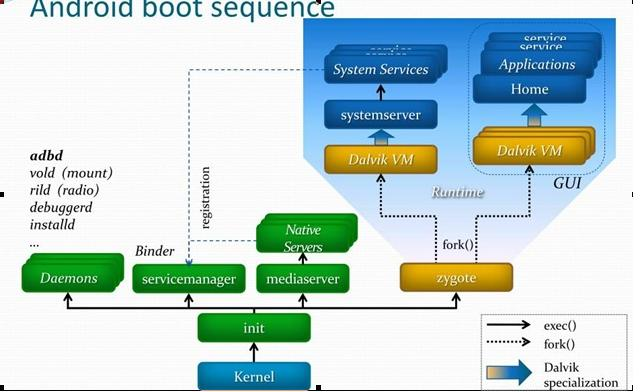
\includegraphics[natwidth=640mm,natheight=392,scale=.3]{bootseq.png}
\end{center}
\caption{{\bf Android boot sequence}} 
\label{figzygote}
\end{figure}



We found that virtually all processes need to read from \verb|/dev/urandom| at their start. We looked into why and found that recent Android versions since 4.0 adopted the stack protector mechanism, as known as stack canaries to protect the Android framework processes as well as native code bridged by Java Native Interface in user applications.

The stack protector works with the help of two components:
\begin{itemize}

\item Android NDK compiler (gcc): insert putting and checking code in function prologues and epilogues. The canary value is read from a global variable.
\item The standard C library (bionic): initialize the canary value by reading 4 bytes from \verb|/dev/urandom| and put it in a global variable. The initialization routine is a library constructor which is invoked by the dynamic linker after mapping the shared library into the process? memory space, typically when the process is exec()ed.
\end{itemize}

However, the way in which the canary value is initialized could be problematic on Android platform. All system services and user applications running on the Dalvik VM are forked from a process called Zygote. By leveraging the Copy-on-Write fork on Linux, Android apps do not need to load the Dalvik VM execution image or the shared library repeatedly on start, leading to better performance. But it also means that there is no chance for an app to invoke the library constructor which setup the canary value. Therefore all Android processes share one stack canary.

We made an app \cite{jnioverflow} to show its canary value on the screen and compared this value to what \verb|app_process| (which then forked Zygote) read from \verb|/dev/urandom| on its start. The result verified this vulnerability. 

\subsubsection{Predictable Stack Canary}

Combining section 2.2 and 2.3, we found that it is possible to predict the canary value shared by all Android apps and Zygote. Note that EntropyMixer is also a system service running on Dalvik VM and thus is going to be forked from Zygote. Therefore, when Zygote sets up its canary value, the \verb|/dev/urandom| is only initialized by its internal routine (\verb|std_initialise|)  with the system information and boot time.

However in our experiment, we found the canary value was not a constant when the initial state of \verb|/dev/urandom| pool was fixed. 

We conjectured that it was due to multitasking and different scheduling realization, because \verb|/dev/urandom| adopts a fine grained locking scheme that maximizes parallelism. It is possible that the internal state changes during the current reading process is descheduled. To verify our conjecture, we modified the \verb|/dev/urandom| interface to enforce a coarse grained locking scheme so that other process cannot change the internal state before the current process finishing reading. It then showed a fixed canary value that depend only on the initial state of \verb|/dev/urandom|.

Given no entropy mixed into the pool of \verb|/dev/urandom|, the internal state depends only on the number of extractions from the pool (this is different from the number of bytes read from \verb|/dev/urandom|, because the minimum number of bytes to extract is 10). With the non-determinism of scheduling, we can model the canary value as a function $f(B,N)$ where $B$ is the boot time and $N$ is the number of extractions from \verb|/dev/urandom| that happened before Zygote read from it.


$B$ is acquired by \verb|getnstimeofday()| function which supports resolution of nanosecond, but we observed only microsecond precision on our devices.
$B$ may not confirm to a specific distribution and the attacker may have knowledge about it in various degrees, we can only make some simple assumption, for example, we can assume that the attacker knows the boot time with precision of second, then the attacker has to guess the microsecond out of $10^6$ values, equivalent to 20 bits of entropy.

$N$ may confirm to some distribution because it can be seen as a value affected by a set of independent events. In order to characterize its distribution, we collected its realization from 244 times of boot; the result is shown in figure \ref{fighist}.

\begin{figure}[t]
\begin{center}
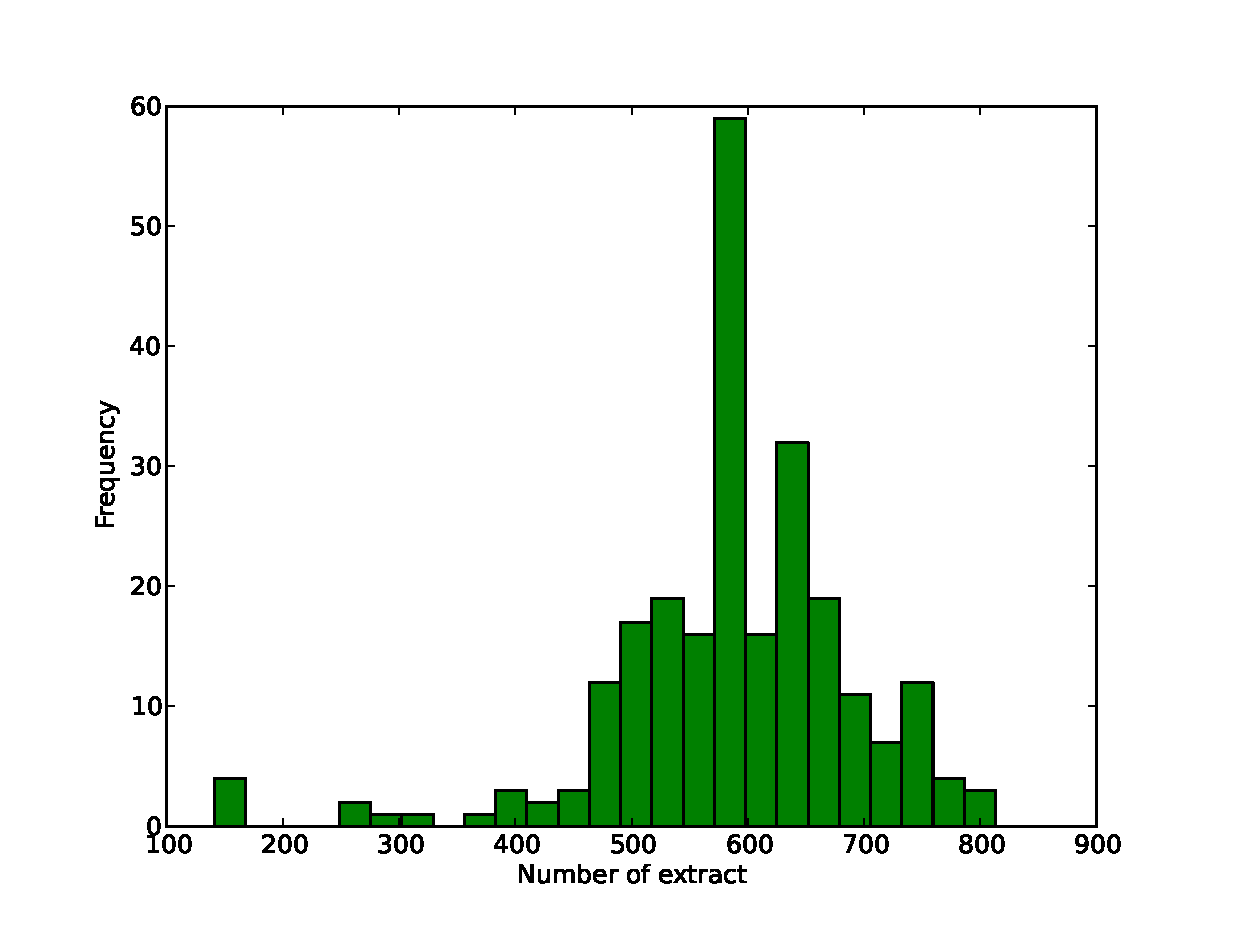
\includegraphics[scale=0.4]{hist.eps}
\end{center}
\caption{{\bf Histogram of number of extractions from \texttt{/dev/urandom} before Zygote runs:} we repeatedly reboot a Nexus 7 for 244 times to record the number of extractions. The result suggests a bell curve distribution of the data which could help the attacker guess the canary value more effciently }
\label{fighist}
\end{figure}

If the attacker has prior knowledge of this distribution of the number of extractions before, he could guess the ranges in a higher probability first order, which gives an expected number of guess of 133 in our case, equivalent to about 7 bits of entropy.

%XXX Entropy estimation!!

With the above model, we can estimate that $B$ and $N$ together will provide 27 bits of entropy, assuming the attacker knows the boot time in second.

Although the computation needed to predict the value of canary may be comparable to simply guessing the 32-bit canary, this vulnerability nullifies the additional security brought by extending the length of the canary. Furthermore, the system time is not a secret number and can be leaked via various ways.

\subsubsection{Nullified ASLR}

Since 4.0, Android has turned on address space layout randomization with the support of the kernel. Despite of only 8 bits of entropy is added for each mapped region, due to the fork nature of Zygote, all Android apps share one address layout, including the same base addresses of the stack, the heap and the standard C library.

